% !TEX root = defense_index.tex

\begin{center}
Those who fail to plan, plan to fail.
\par Attributed to Benjamin Franklin
\end{center}

The application of \acp{IV} on \acp{EEG} is a novel concept given that \acp{IV} were designed for speech processing. Therefore, there is minimal guidance on how to use \acp{IV} on \ac{EEG} data. As indicated in the background, the foundations of the experiments proposed here came from following the development of \acp{IV} within the speech community. The two fields are related in terms of their signal analysis goals, and subject and condition discrimination (Research Aim 1), but their optimization processes may be different (Research Aim 2). In both Aims, the desired goals afford insight into the classification process, which in turn is leveraged into insight about the features, datasets, and \acp{EEG} themselves.

%%%%%%%%%%%%%%%%%%%%%%%%%%%%%%
\section{Experimental Outline}

The ultimate goal of this research is to provide subject and condition discrimination of \acp{EEG}. Prior to this work, this goal was not possible using \acp{IV} given the lack of a software tools specifically for \acp{EEG}. The first experiments provided classification performance showing that \acp{IV} met or exceeded performance of equivalent techniques. Providing competitive classification required an understanding of the technique's trade-offs in terms of features, datasets, and parameters. Running experiments to sweep through the features, datasets, and parameters provided operational thresholds for the datasets, \acp{UBM}, and \acp{UBM} for using \acp{IV} based classification on \acp{EEG}.

In this work the experiments are classified as \emph{Algorithm Benchmarks}, \emph{Parameter Sweeps}, and \emph{\ac{UBM}-\ac{TVM} Relationship}. The Algorithm Benchmarks addressed \ac{RA1} by testing the performance of \acp{IV} against benchmark classifiers, specifically Mahalanobis distance and \ac{GMMUBM}. The initial comparisons were carried out using parameters borrowed from speech recognition, which then required optimization through the Parameter Sweeps that addressed \ac{RA2}. Using the optimal classification parameters, the mechansims by which \acp{IV} carried out their classification was resolved through analysis of the relationships between the \acp{UBM}, \acp{TVM}, and feature sets. These \ac{UBM}-\ac{TVM} Relationship experiments addressed \ac{RA3} and represented the major contribution to understanding \acp{EEG} and multi-modal signal analysis.

Each experiment operated on the same fundamental features, datasets, and evaluations as they built upon each other. This chapter details all the components used to build out the experiments. The ensuing three chapters organize present each of the experiments: \Cref{chap:5} - Parameter Sweeps, \Cref{chap:6} - Algorithm Benchmarks, and \Cref{chap:7} - \ac{UBM}-\ac{TVM} Relationship.

%%%%%%%%%%%%%%
\section{Data}

Using heterogeneous data is necessary for validating any statistically rigorous method such as \acp{IV}, but \ac{EEG} data is difficult to obtain. Typically, new data is generated as part of research experiments and/or acquired from hospitals, but rarely if ever enters the public domain. This limits innovation to specific combinations of data and techniques. To mitigate this, only the publicly available datasets from \ac{PNET}\cite{Goldberger2000} and \ac{TUHEEG}\cite{Obeid2016a} were used in this work. While not comprehensive in terms of the variety of subjects and conditions used in other studies this collection provided the necessary breadth to validate the goals of this work. These data include \ac{EEG} from imagined and actual hand, arm, and foot motion, and normal, abnormal, and seizure clinical \acp{EEG} from over 600 subjects.

%%%%%%%%%%%%%%%%%%%%%%%%%%%%%%%
\subsection{PhysioNet Database}

This \ac{EEG} data comes from the New York State Department of Health's Wadsworth Center \cite{Schalk2004} and is a component of the PhysioBank archive maintained by MIT's Lab for Computational Physiology\footnote{https://www.physionet.org/pn4/eegmmidb/}. Within the data bank are \ac{EEG} recordings pertaining to resting states, imagined motion, and motion tasks. The \sout{collected} data consist of 64 channel \acp{EEG} from 109 subjects performing 14 trials: 12 motion and 2 resting calibration (see Figure \ref{fig-chap3_physioTasks}). Information about the subjects (age, gender, handedness, etc) is not provided, making subjects and trials the most applicable decision surfaces.


\begin{figure}
\centering
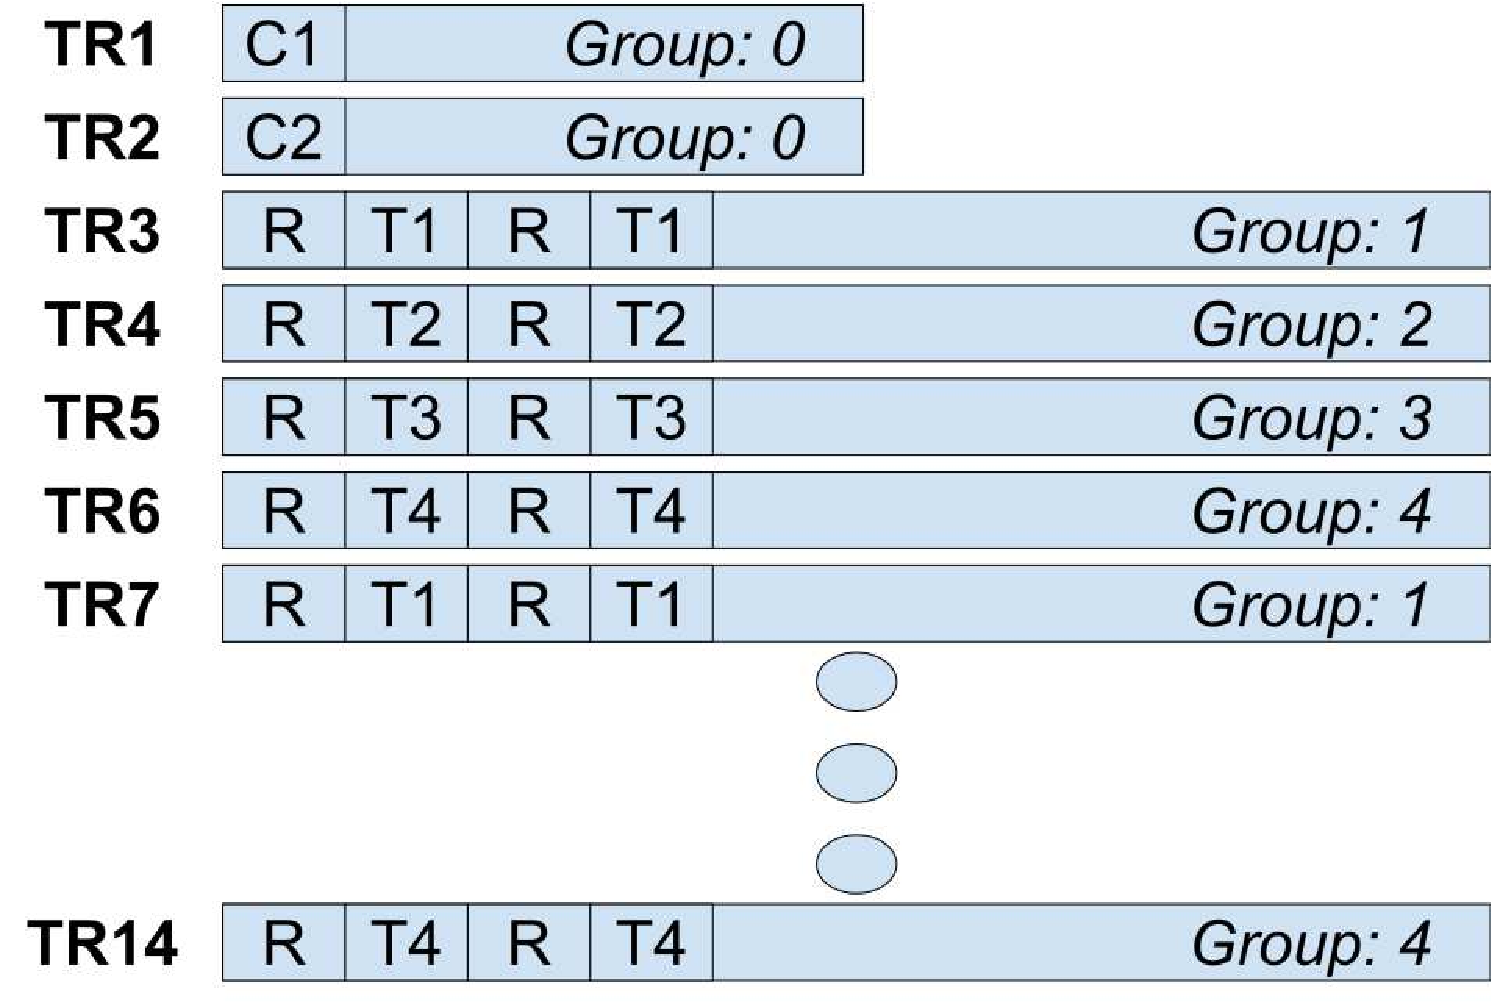
\includegraphics[width=0.7\linewidth,keepaspectratio]{physioTasks}
\caption[Format of PhysioNet Trials]{The 12 \acf{PNET} trials are broken down by their tasks into 2 resting trials (TR1, TR2) and the four imagined-motion/motion trials (TR3-TR14). This provided depth for subject evaluation, by adding trials, but also for within subject trial evaluation as the repeated trials could be grouped.}
\label{fig-chap3_physioTasks}
\end{figure}

Each 2-minute imagined-motion/motion trial consists of a series of 30 4.1 second tasks. These alternate between rest states and the computer prompted tasks (T1-T4). The tasks consist of opening/closing left or right fist (T1), imagine opening/closing left or right fist (T2), opening/closing both fists or feet (T3), and imagine opening/closing both fists or feet (T4). The two resting state trials, TR1 \acf{EO} and TR2 \acf{EC}, are one minute recordings of unprompted subject recordings. From this, three dataset 

\begin{enumerate}
\item \textbf{Physio Full} -  All fourteen trials (TR01-TR14)
\item \textbf{Physio Single} - One trial of each type (TR01-TR06)
\item \textbf{Physio Motion} - One of each motion trial (TR03-TR06)
\end{enumerate}

These datasets allowed classification experiments on distinct levels of the data. The highest level was subject classification across trials. Beneath that was subject-trial classification, dependent on matching the correct subject and trial. Finally, within-subject trial classification was possible given the grouping of the repeated trials.

The recordings consist of 64 electrodes sampled at 160Hz following a standard 10-20 layout. A 65th channel provides labels for each task during the trials. Since its introduction in 2009, the \ac{PNET} has been used in biometric classifications \cite{Delpozo-Banos2015} with respect to task sensitivity \cite{Yang2016}, subject independence \cite{Reuderink2011}, various subject classification schemes \cite{Fraschini2015,Rodrigues2016}, and attempts at content based retrieval \cite{Su2013a}.

%%%%%%%%%%%%%%%%%%%%%%%
\subsection{TUH Corpus}

The \acf{TUHEEG} contains over 25,000 \acp{EEG} with their associated medical evaluations. All data comes from patients seen by Temple University Hospital in Philadelphia, Pennsylvania \cite{Obeid2016a}. These recordings represent considerable breadth and depth in terms of patients, medical conditions, and recording conditions. Seizures were the most common diagnosis for patient's with medical records, but stroke and concussion patients are represented as well, while the majority of all recordings are simply indeterminate. In addition to these patients, there are subsets consisting of normal patients and those with indeterminate conditions considered abnormal. These latter classifications (abnormal/normal) along with seizure patients were used to organize 3 distinct datasets:

\begin{enumerate}
\item \textbf{TUH Normal} - 50 normal patient sessions
\item \textbf{TUH Abnormal} - 50 abnormal patient sessions
\item \textbf{TUH Seizure} - 411 seizure patient sessions
\end{enumerate}

These datasets allowed for two types of classification experiments. The first was on the subject level, as each was built from unique subjects. The second was developed by combining the datasets to classify them based upon their condition, abnormal/normal/seizure. Further analysis was possible given the associated medical reports, but beyond the time and scope of this research.

%%%%%%%%%%%%%%
% figure of TCP montage, CEP
%%%%%%%%%%%%%%
\begin{figure}
\centering
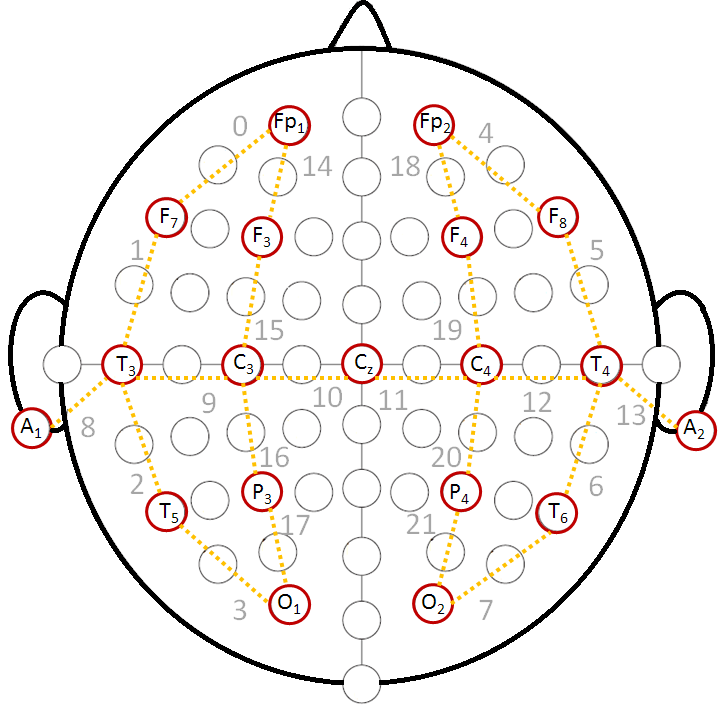
\includegraphics[width=7cm,keepaspectratio]{figure3}
\caption[Layout of \acs{TCP} montage for \acs{CEP} features.]{The \acf{TCP} montage uses a rostral to caudal differential between electrodes to produce channel data. This differential is applied from the ears inward as well to produce 22 distinct channels. Common electrode names are provide with intermediate electrodes left blank. The gray numbers represent the channel index found in the \acf{TUHEEG}.}
\label{fig-chap3_tcpMontage}
\end{figure}
%%%%%%%%%%%%%

Unlike the \ac{PNET}, the \ac{TUHEEG} is \emph{in vivo}, leading to a wide array of recording variation. The electrode configurations, sampling rates, and session counts are at the discretion of medical professionals and not a structured research protocol. As addressed in its public release \cite{Obeid2016a}, the most common recording configuration consists of 31 electrodes at a 250Hz sample rate. This is substantially fewer electrodes than the \ac{PNET}, but is enough to produce clinically common \ac{EEG} montages\footnote{ACNS - Guideline 3: \url{http://www.acns.org/UserFiles/file/EEGGuideline3Montage.pdf} }.

%%%%%%%%%%%%%%%%%%%%%%%%%%%%%%
\subsection{Synthetic Dataset}
\label{chap3:syn}

Developing and testing on experimental data alone would make it impossible to provide validation of the software's efficacy; therefore, a synthetic dataset was built. This controlled dataset allowed for two `ideal' configurations: (1) a dataset with a common feature across all subjects and (2) a dataset with an unique feature for each subject. These datasets were labeled as \textit{simulated}, \textit{static} (simulated with an additional common feature across subjects) , and \textit{unique} (simulated with a unique feature for each subject). Each one contained 10 minutes of data for the simulated 12 subjects and their 22 channels, matching the number of channels in the AutoEEG dataset.

Production of the synthetic datasets relied on a \ac{GMMHMM} consisting of 3, 4, or 5 Gaussian models drawn from \acp{UBM}. The baseline \ac{UBM} came from 12 \ac{TUHEEG} AutoEEG V1.1.0 subjects using a 16-mixture \ac{UBM}. The common and unique features came from a single random subject in the \ac{PNET}, also using a 16-mixture \ac{UBM}. Simulated data contained either 3 or 4 mixtures, allowing the static and unique to add an additional feature containing 4 or 5 mixtures depicted by Figure \ref{fig-simData}. 


%%%%%%%%
% figure of synthetic dataset construction
%%%%%%%%
\begin{figure}[!t]
\centering
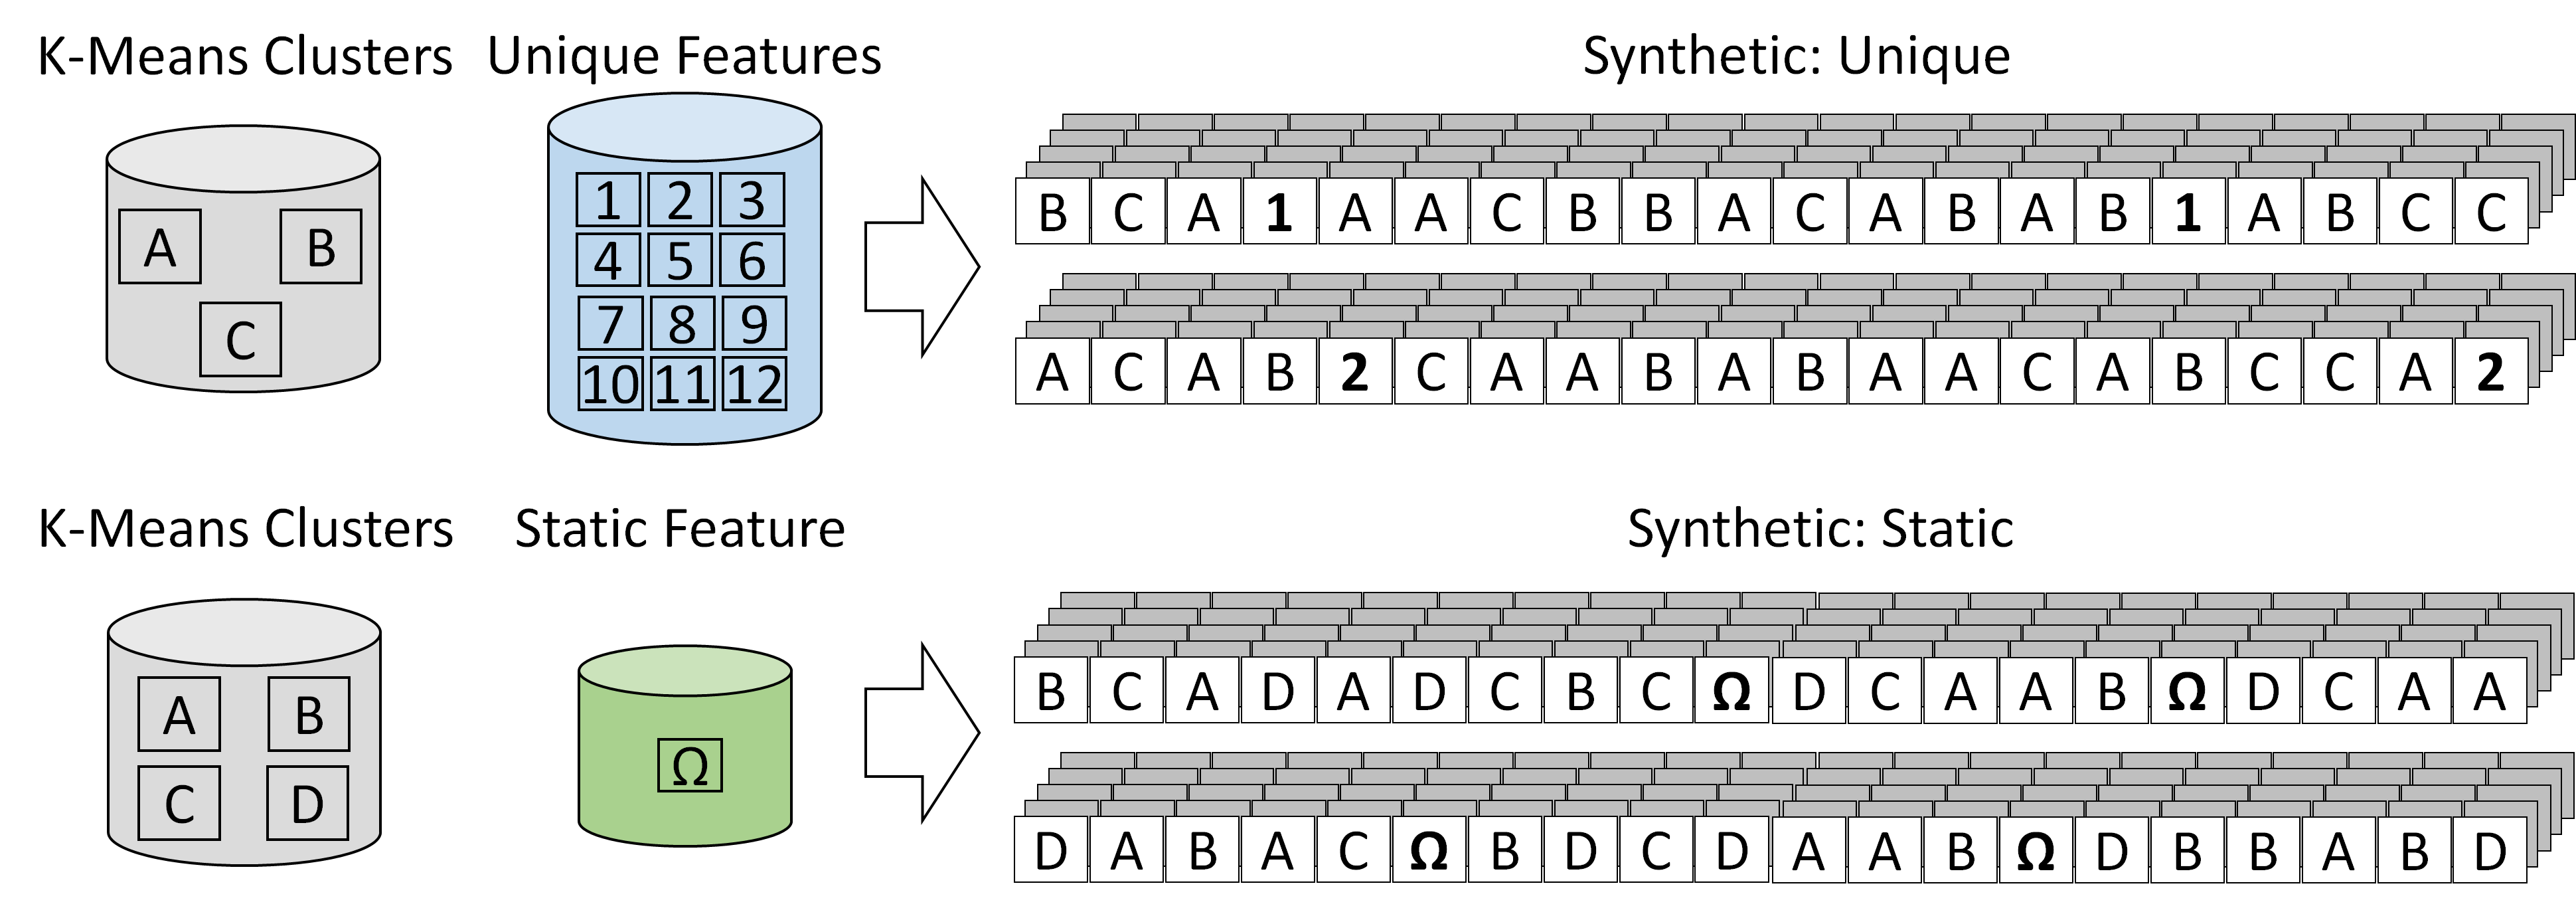
\includegraphics[width=0.7\linewidth,keepaspectratio]{physioSyn}
\caption[Generation of synthetic data from the \acs{TUHEEG}.]{The \ac{GMMHMM} modeled data (gray) and the unique (blue) or static (green) features enable the creation of unique and static synthetic data sets. Only 10\% of the simulated data is replaced by the external \ac{PNET} feature. The modeling produced features for each epoch's 22 channels simultaneously to keep the channel-epochs temporal synchronized for each of the 12 simulated \ac{TUHEEG} subjects.}
\label{fig-simData}
\end{figure}
%%%%%%

This produced six unique synthetic data sets: Sim3, Sim4, Sta3, Sta4, Uni3, Uni4, outlined in Figure \ref{fig-simData}. Data was generated for each one-second epoch of each channel as \ac{CEP} features directly. The distribution of the simulated data followed the weighting of the initial 16 mixture \ac{UBM}. When the static and unique features were added they overwrote 10\% of the simulated data with the new \ac{PNET}-based feature. Authenticity of the raw data was preserved by keeping the synthetic data as similar to the \ac{TUHEEG} AutoEEG V1.1.0 dataset as possible, highlighted in Table \ref{tab-sim_sets}.

%%%%%%%%
% table of synthetic datasets
%%%%%%%%
\medskip
\noindent\makebox[\columnwidth][c]{%
\begin{minipage}{\linewidth}
\centering
\captionsetup{justification=justified, singlelinecheck=false}
\captionof{table}{Composition of Synthetic Data Sets}
\label{tab-sim_sets}
\resizebox{\columnwidth}{!}{%
\begin{tabular}{l c c c c r}
\specialrule{0.2em}{0.1em}{0.1em}
Name & Type & Features & Channels & Sampling Rate (Hz) & Duration (s) \\
\specialrule{0.1em}{0.1em}{0.1em}
AutoEEG & Real & $\infty$ & 22 & 100 & 1200 \\
PhysioNet & Real & $\infty$ & 64 & 160 & 120 \\
\specialrule{0.1em}{0.1em}{0.1em}
Sim3 & Simulated & 3 & 22 & 100 & 600 \\
Sta3 & Static & 4 & 22 & 100 & 600\\
Uni3 & Unique & 4 & 22 & 100 & 600\\
\specialrule{0.1em}{0.1em}{0.1em}
Sim4 & Simulated & 4 & 22 & 100 & 600\\
Sta4 & Static & 5 & 22 & 100 & 600\\
Uni4 & Unique & 5 & 22 & 100 & 600\\
\specialrule{0.2em}{0.1em}{0.1em}
\end{tabular}
}
\end{minipage}}
\medskip
%%%%%

%%%%%%%%%%%%%%%%%%%%%%%%%
\subsection{Feature Sets}

In addition to using multiple datasets, three feature sets were applied to the \ac{PNET} and \ac{TUHEEG}: \acf{CEP}, \acf{COH}, and \acf{PSD}. Using multiple feature sets was important because there is no consensus on an optimal feature set for \acp{EEG}. \ac{PSD} features have a long history of use with \acp{EEG} \cite{Lotte2007b,Dymond1978,Berka2007}, as do \ac{COH} features \cite{Rocca2014,Ruiz-blondet2016}. \ac{CEP} are well-established features in the speech processing domain \cite{Furui1981,Li2013a}; their application to EEG research was introduced by the \ac{NEDC} \cite{Harati2015a}. 

The \ac{COH} and \ac{PSD} features were computed according to the work of LaRocca \cite{Rocca2014}. The \ac{CEP} features were built following the standards developed by the speech community \cite{Harati2015a} and their channels modified to conform with a \ac{TCP} montage used by neurologists \cite{Lopez2015}. Thus the feature sets are distinct not only in their mathematical construction, but also their topographical configurations, Table \ref{tab-feat_sets_config}. 

%%%%%%%%%%%%%%
% table of features
%%%%%%%%%%%%%%
\medskip
\noindent\makebox[\columnwidth][c]{%
\begin{minipage}{0.5\linewidth}
\centering
\captionsetup{justification=justified, singlelinecheck=false}
\captionof{table}{Feature Set Configurations}
\label{tab-feat_sets_config}
\resizebox{\columnwidth}{!}{%
\begin{tabular}{l c c c}
\specialrule{0.2em}{0.1em}{0.1em}
Name & Type & Features & Channels \\
\specialrule{0.1em}{0.1em}{0.1em}
%
\multirow{2}{4em}{CEP} & Original & 26 & 22 \\
& Slim & 26 & 22\\
\midrule
%
\multirow{2}{4em}{PSD} & Original & 40 & 56 \\
& Slim & 40 & 19 \\
\midrule
%
\multirow{2}{4em}{COH} & Original & 40 & 1540 \\
& Slim & 40 & 22 \\
\specialrule{0.2em}{0.1em}{0.1em}
\end{tabular}
}
\end{minipage}
}
\medskip
%%%%%%%%%%%%% 

As discussed in the background, \ac{EEG} recordings can use a variety of electrode configurations. For example, the \ac{PNET} contains 64 electrodes of data, while the \ac{TUHEEG} contained a myriad of electrode configurations. Therefore the \ac{TUHEEG} set was aligned with the most common standard, the \ac{TCP} montage, resulting in 19 electrodes organized as 22 differential channels. La Rocca's features consisted of 56 \ac{PSD} channels and 1540 \ac{COH} channels making for a larger disparity in channels for each feature set. To address this channel imbalance, the \ac{TUHEEG} configuration layout was replicated for the \ac{PSD} and \ac{COH} feature sets producing two groups of features. The first was the 55 electrode layouts used by La Rocca \cite{Rocca2014} and the second time was a mirror of the 19 electrodes from the \ac{TUHEEG} \ac{TCP} montage.

This resulted in a slim feature set consistent of the 22 channel \ac{CEP}, 19 channel \ac{PSD}, and 22 channel \ac{COH}. The \ac{CEP} and \ac{COH} confirmed to the \ac{TCP} layout, but the \ac{PSD} were not converted to keep them as distinct from the \ac{COH} features as possible. The benchmark testing against La Rocca's worked used the full feature sets, while all Algorithm Benchmarks and \ac{UBM}-\ac{TVM} Relationship experiments used the slim feature sets.

%%%%%%%%%%%%%%%%%%%%%%%%%%%%%%%%%
\subsubsection{Cepstral Features}

The \ac{CEP}-based features were predicated on the success of similar \ac{MFCC} used in speech recognition. Their adoption for \ac{EEG} required shifting from a log frequency scale to linear frequency and adjusting the time windows for the $\Delta$ and $\Delta\Delta$ differentials. Generation of these features was introduced and detailed by Harati et al in \cite{Harati2015a}, but is outlined here.

The base feature vector consisted of of nine coefficients (seven cepstral coefficients, the frequency domain energy, and the differential energy). The filter banks actually produce eight spectral coefficients covering the following frequency ranges: \{0, 1-10, 11-20, 21-30, 31-40, 41-50, 51-60, 71-80 Hz\}. However, the zeroth coefficient is discarded and replaced with the frequency domain energy; the differential frequency energy becomes the ninth term. These filters provided a single energy value after bandpass filtering (Hamming) the \ac{FFT} for each of the listed frequency ranges.

The two energy terms: frequency domain ($E_{f}$) and differential frequency energy ($E_{d}$) are given as:
\begin{equation}
E_{f} = \text{log}\Big( \sum_{k=0}^{N-1}\absv{X(k)}^2 \Big)
\end{equation}
\begin{equation}
E_{d} = \text{max}\Big( E_{f}(m) \Big) - \text{min} \Big( E_{f}(m) \Big)
\end{equation}
$E_{f}$ was derived from the outputs of the filter banks where $N$ are the number of filters and $X$ is the filtered cepstrum frequency output. Using these values within the prescribed 0.9s window of samples, the $E_{d}$ is found by comparing the maximum and minimum $E_{f}$ values over the range of $m$ elements in the signal window. These built the first nine features with the remaining 17 coming from the first derivative ($\Delta$) and second derivative ($\Delta\Delta$).

The $\Delta$ and $\Delta\Delta$ features used the same equations, but with different window sizes:
\begin{equation}
d_{t} = \frac{\sum_{n=1}^{N}\big[ c_{t+n}--c_{t-n} \big]}{2\sum_{n=1}^{N}n^{2}}
\end{equation}
Here each sample $n$ in the window $N$ was used to produce a derivative for a given coefficient $c$ centered around time $t$. Zero padding was used to pad the vector near the beginning and ending of the data. The first derivative $\Delta$ used $N=0.9$. Once resolved, the second derivative $\Delta\Delta$ used the $\Delta$ values with a new window of $N=0.3$. In Harati's work \cite{Harati2015a}, the optimal configuration was found to be a 26 feature vector where the $\Delta\Delta$ for $E_{d}$ was excluded. This configuration was adopted by the research group and became the consistent feature for the experiments in this work.

%%%%%%%%%%%%%%%%%%%%%%%%%%%%%%%%%%%%%%%%%%%%%%%
\subsubsection{Power Spectral Density Features}

\ac{PSD} features are derived from the sum of energy over a frequency range for a given time sample. Variation in their creation can be found in their frequency range, number of \ac{FFT} samples, and filtering of the time signal. The variation of \ac{PSD} based features used in this work are identical to those of La Rocca et al. \cite{Rocca2014} which used a frequency range of 0-100Hz, a 100-point \ac{FFT}, and Hanning windows for filters. The final features were 10-second epochs with 40 \ac{PSD} values evenly spanning 1-40Hz.

The time series data was filtered with 1 second Hanning window using a 0.5 second overlap. This produced 20 filtered samples for each 10 second epoch centered around each 1 second interval from 0 to 9.5 seconds. These filtered samples were evaluated using Welch's averaged modified periodgram (built into Matlab) with a 100 point \ac{FFT} to produce 1Hz resolution over the range of 0 to 100Hz. La Rocca's work used the \ac{PNET} data which first had to be resampled from 160Hz to 100Hz prior to the filtering.

The resultant 100 energy levels were reduced down to only those spanning 1-40Hz. This reduction in frequencies is necessary given (a) the resampling and (b) that the \ac{EEG} oscillations of interest Delta (0.5-4Hz), Theta (4-7Hz), Alpha (8-14Hz), Beta (15-29Hz), and Gamma (30-40Hz) fall within that range. This resulted in 40 features per \ac{EEG} channel. The channel count was reduced to 56 from \ac{PNET}'s original 64. The discarded channels, highlighted in Figure \ref{fig-chap3_roccaLayout}, were AF\textsubscript{7}, AF\textsubscript{8}, FT\textsubscript{7}, FT\textsubscript{8}, T\textsubscript{9}, T\textsubscript{10}, O\textsubscript{Z}, and I\textsubscript{Z}.

%%%%%%%%%%%%%%
% figure of Rocca Channels
%%%%%%%%%%%%%%
\begin{figure}
\centering
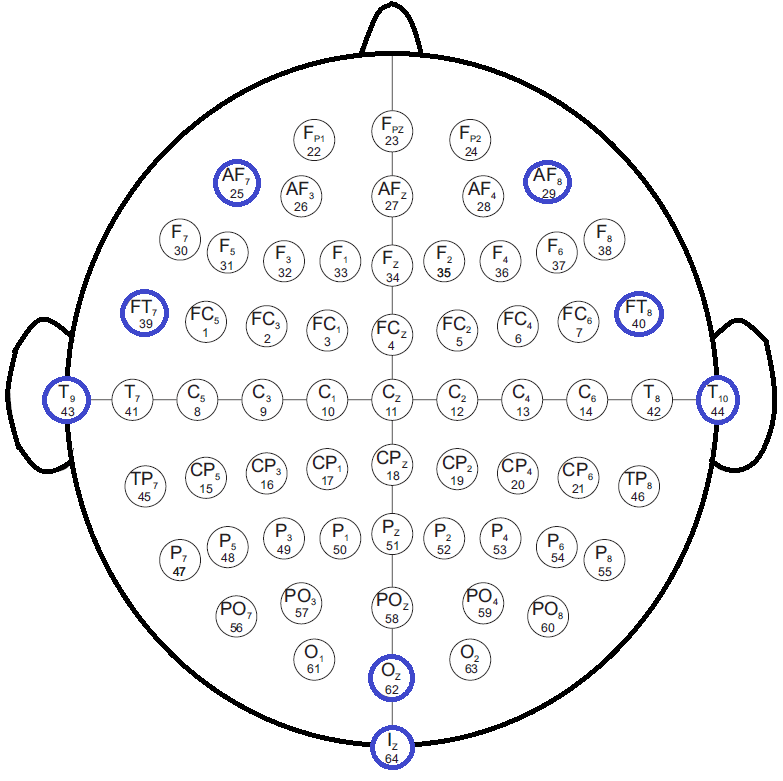
\includegraphics[width=7cm,keepaspectratio]{rocca_layout}
\caption[Layout of La Rocca's PSD and COH Channels.]{The channel layout La Rocca et al used removed 8, highlighted in blue, channels from the overal 64 channel configuration of the \ac{PNET}.}
\label{fig-chap3_roccaLayout}
\end{figure}
%%%%%%%%%%%%%

While originally designed with the \ac{PNET} in mind, these features were readily adapted to the \ac{TUHEEG}. Recordings were resampled to 100Hz and pared down to the match the abbreviated 56 channel layout.

%%%%%%%%%%%%%%%%%%%%%%%%%%%%%%%%%%%%%%%%%%%
\subsubsection{Spectral Coherence Features}

The \ac{COH} features were proposed by La Rocca as an improvement  over \ac{PSD} features for subject classification. Measuring coherence between electrodes had been used prior for distinguishing \ac{ADHD} \cite{Monastra2001}, a general connectivity measure of the brain \cite{Makeig2012} and auditory oddball paradigms for \ac{BCI}/P300 responses \cite{Guntekin2016}. Thus they were not novel features, but applied to a broad range of applications beyond subject classification.

These features were generated by quantifying the amount of synchronous energy at each frequency band of each electrode. This was achieved by first building the \ac{PSD} features and then using them to generate a \ac{COH} value for each frequency $f$ between two different electrodes $i$ and $j$, outlined as follows:
\begin{equation}
\text{COH}_{i,j}(f) = {\frac{\absv{S_{i,j}(f)}^{2}}{S_{i,i}(f) \cdot S_{j,j}(f)}}
\end{equation}
The resultant values were scaled by arctan to normalize their distribution making them bounded on the range $(0,\frac{\pi}{2})$. This configured the final feature set as 1540 `channel' which La Rocca called elements. Each with the 40 distinct frequency bins found through the \ac{PSD} feature process.

%%%%%%%%%%%%%%%%%%%%%%%%%%%%%%%%%%%
\subsubsection{Aggregated Datasets}

The \ac{UBM}-\ac{TVM} Relationship experiments needed subject and condition variation to test classification performance. To achieve, this aggregated datasets were built by combining the \ac{PNET} and \ac{TUHEEG} datasets. The combinations of \ac{PNET}'s motion data and the \ac{TUHEEG}'s normal, \ac{TUHEEG}'s abnormal and normal, or \ac{TUHEEG} abnormal, normal, and seizure datasets allowed classification of subjects and known characteristics within a single experiment. This was important to address algorithm robustness and to mitigate any benefits conferred based upon a given dataset-feature-algorithm combination. Each combination was given a designation, Table \ref{tab-dataset_desig} to streamline documentation and discussion.

%%%%%%%%%%%%%%
% table of features
%%%%%%%%%%%%%%
\medskip
\noindent\makebox[\columnwidth][c]{%
\begin{minipage}{0.7\linewidth}
\centering
\captionsetup{justification=justified, singlelinecheck=false}
\captionof{table}{Combine Dataset Designations}
\label{tab-dataset_desig}
\resizebox{\columnwidth}{!}{%
\begin{tabular}{l c c c}
\specialrule{0.2em}{0.1em}{0.1em}
Designation & Dataset 1 & Dataset 2 & Dataset 3 \\
\specialrule{0.1em}{0.1em}{0.1em}
%
\AbnNrm{} & TUH Abnormal & TUH Normal & - \\
\AbnSzr{} & TUH Abnormal & TUH Seizure & - \\
\NrmSzr{} & TUH Normal & TUH Seizure & - \\
\midrule
\AbnMot{} & TUH Abnormal & Physio Motion & - \\
\NrmMot{} & TUH Normal & Physio Motion & - \\
\SzrMot{} & TUH Seizure & Physio Motion & - \\
\midrule
%
\AbnNrmSzr{} & TUH Abnormal & TUH Normal & TUH Seizure \\
\AbnNrmMot{} & TUH Abnormal & TUH Normal & Physio Motion \\
\NrmSzrMot{} & TUH Normal & TUH Seizure & Physio Motion \\
\AbnSzrMot{} & TUH Abnormal & TUH Seizure & Physio Motion \\
\specialrule{0.2em}{0.1em}{0.1em}
\end{tabular}
}
\end{minipage}
}
\medskip
%%%%%%%%%%%%%

%%%%%%%%%%%%%%%%%%%%%%%%%%%%
\section{Evaluation Metrics}

All experiments were run as subject verification tests. This was inline with La Rocca's experiment which used \ac{CRR} as their sole evaluation metric. However, given the depth of the datasets and parameter testing to be conducted it was necessary to also include the \ac{EER} as well. The performance of \acp{IV} has typically been reported in terms of \ac{EER}, while the \ac{EEG} research community is typically more broadly focused more on \ac{CRR}. Exceptions in the literature \cite{Yang2016, Marcel2007a, Nguyen2013} show results in terms of \ac{EER}, \ac{FAR}, \ac{FRR}, \ac{HTER}, or \ac{DET} curves. For the purposes of this research results were reported in terms of \ac{CRR} and \ac{EER} to facilitate readers from both the \ac{IV} and \ac{EEG} communities being able to contextualize the experiment performances.

In this work \ac{CRR} was calculated based on the testing data correctly matching into the enrollment data. The \ac{EER} was calculated over the entire distance matrix ensuring it evaluated the strength of all matches. This meant if subject 100s second best score was stronger than subject 4's score the \ac{EER} would be none zero. This is why it was critical to include it for the parameter sweeps, as the \ac{CRR} masked the majority of the nuance of the full system.

Even with the importance of both metrics, the intended parameter sweeps and comparison points made always displaying both \ac{CRR} and \ac{EER} cumbersome and ineffective to the end goal of comparative performance. AS such, the C Metric was defined which combined the \ac{CRR} and \ac{EER} by subtracting the \ac{EER} from the \ac{CRR}. Thus the threshold for an acceptable C Metric score was set at 0.75 which could represent a \ac{CRR} of 85\% and an \ac{EER} of 10\%. This was primarily used for the expansive Algorithm Benchmarks to showcase performance differences between \acp{GMMUBM}, \ac{MD}, and \acp{IV}.

%%%%%%%%%%%%%%%%%%%%%%%%%
\subsection{Mixture Size}

For \acp{UBM}, \acp{TVM}, and \acp{IV} the dimension of the underlying mixture model is a critical parameter than can affect performance. Effectively, the n dimensional feature space is modeled by m gaussians; these gaussians are used to train the \acp{IV}. As has been the case in the speech community \cite{Bahari2012, Glembek2011, Behravan2013}, it was necessary to determine the size of the mixture model that would optimize \ac{IV} performance under different circumstances. While some experiments applied \acp{GMMUBM} previously, their protocols and datasets were not a sufficient starting point\cite{Marcano2018, Nguyen2013}.

These experiments were used to inform the initial mixture sweep range \{2, 4, 8, 16. 32, 64, 128, 256, 512, 1024\} used as part of the Parameter Sweeps. After which it was expanded to \{2, 4, 8, 16, 32, 64, 128, 256, 512, 1024, 2048\} for the Algorithm Benchmarks and \ac{UBM}-\ac{TVM} Relationship experiments. The smallest datasets contained 50 subjects, but each dataset had at least 19 channels per subject amounting to a lower bound of 950 distinct subject-channels each with 40 features. From this lower subject-channel bound there the number of epochs in the training and enrollment datastets would change based upon the epoch duration. With the largest epoch duration of 10 seconds, there would be at minimum 9 epochs for each of the 950 subject-channels producing 8,550 unique subject-channel-epochs to model. This value exceeded the upper limits of the two mixture sweeps ensuring overfitting was not a major influence on performance.

%%%%%%%%%%%%%%%%%%%%%%%%%%%
\subsection{TVM Dimensions}

The size of the \ac{TVM} was bounded by the number of mixtures and a depth factor called $l$ from section \ref{2-mathematics}. As stated, this $l$ value had to be less than or equal to the number of subjects, otherwise models would be built specifically for each subject. Overfitting concerns were addressed with respect to the mixture sizes, but limiting the \ac{TVM} depth to the number of subjects assured overfitting was impossible in the production of \acp{IV}.

This was not strictly required, as the examples used to inform this work would build \acp{TVM} with a depth beyond that of the number of subjects \cite{Dehak2011}. As the \ac{TVM} is an intermediate step before finalizing the \acp{IV} with \ac{LDA}, the dimension of the \ac{TVM} could be 1200 for processing data from 75 subjects \cite{McLaren2011}. However, such options were based on datasets with an order of magnitude more epochs and contained feature vectors double in size than was proposed in this work

Bounding the upper limit was necessary given the dynamic between mixture size, \ac{TVM} depth, and \ac{LDA} depth. An upper bound of 200 was chosen because the majority of datasets and aggregated datasets would not exceed 200 subjects. Additionally, producing the \ac{TVM} was the most computational intense components of the algorithm requiring a tradeoff of the sweep range and execution time. The lower bound was set at 25, half the smallest subject count. Three incremental values were used to step between the lower and upper bound which resulted in the following sweep range: \{25, 50, 75, 100, 200\}.

%%%%%%%%%%%%%%%%%%%%%%%%%%
\subsection{LDA Dimension}

The use of \ac{LDA} to finalize the \acp{IV} was well documented by the founders of \acp{IV} \cite{Dehak2011a,Dehak2011} highlighting their own sweep for optimization with speech data. Thus \ac{LDA} depth represented a third parameter to consider when building and evaluating \ac{IV} performance. The upper bound of \ac{LDA} is determined by the size of its paired \ac{TVM}. As the range of \ac{TVM} dimensions was being aligned with the various aggregated dataset subject counts, the \ac{LDA} dimensions were aligned to operate on a similar scaling.

The lower bound for \ac{LDA} size was set to 15, slightly less than the \ac{TVM} lower bound, and the upper bound was set to 100, half the \ac{TVM} upper bound. Five intermediate values were chosen between the bounds which resulted in the following sweep range: \{15, 30, 45, 60, 75, 100\}. By focusing on smaller increments this parameter was designed to be less influential than the mixture size and the \ac{TVM} depth. This sweep range would later be adjusted following the results of the Parameter Sweeps to: \{5, 15, 20, 25, 25, 50, 75, 95, 100, 150, 195\}.

%%%%%%%%%%%%%%%%%%%%%%%%%%%%%%%%
\subsection{Epoch Configuration}

The final controllable parameters were the number and duration of epochs. Drawing the experiments from the work of La Rocca et al, the initial epoch duration was 10 seconds with 6 epochs per subject, based around the resting trials of the \ac{PNET}. The epoch durations were expanded to include 5, 2, and 1 second epochs. This naturally altered the number of epochs as the \ac{PNET} contained 1 minute and 2 minute trials which split into a various numbers of epochs for each epoch duration recording combination, show in Table \ref{tab-epoch_config}.

%%%%%%%%%%%%%%
% table of epochs
%%%%%%%%%%%%%%
\medskip
\noindent\makebox[\columnwidth][c]{%
\begin{minipage}{0.5\linewidth}
\centering
\captionsetup{justification=justified, singlelinecheck=false}
\captionof{table}[Epoch Duration Configuration]{Number of total epochs per subject as a function of epoch duration.}
\label{tab-epoch_config}
\resizebox{\columnwidth}{!}{%
\begin{tabular}{l | c c c c}
\specialrule{0.2em}{0.1em}{0.1em}
 & \multicolumn{4}{c}{Epoch Duration (s)} \\
\specialrule{0.1em}{0.1em}{0.1em}
 Trial Duration (s) & 10 & 5 & 2 & 1 \\
\specialrule{0.1em}{0.1em}{0.1em}
%
60 & 6 & 12 & 30 & 60 \\
120 & 12 & 24 & 60 & 120 \\
\specialrule{0.2em}{0.1em}{0.1em}
\end{tabular}
}
\end{minipage}
}
\medskip
%%%%%%%%%%%%%

Based upon reviewer feedback to a prior publication \cite{Ward2019} epoch generation was altered to enabled the number of epochs to be independent of epoch duration. This provided another parameter to sweep, number of epochs, which was previously conflated with the epoch duration and trial duration.

%%%%%%%%%%%%%%%%%%%%%%%%%%%%
\subsection{Dataset-Feature}

Every experiment conducted used all three feature sets, but not every combination of datasets was explored. This was because finding an optimal feature set was beyond the scope of the proposed work. There were not enough available resources in terms of datasets, features, and time to satisfy a robust feature search. However, it was understood that the proposed experiments could offer insight into feature selection which is why every experiment used all three feature sets.

Despite this limitation, using all three feature sets for each experiment provided a comparison point for understanding algorithm-dataset performance. It was hypothesized that one feature set would generally outperform the others, independent of data. Variations in relative performance triggered by mixture size, \ac{TVM} depth, \ac{LDA} depth, or epoch settings were used to define areas of interest with respect to these controllable parameters. Additionally, using multiple features mitigated any potential bias generated for stumbling upon an ideal dataset-feature-algorithm combination and being able to identify it as such given the number of dataset-feature-algorithm pairings.

%%%%%%%%%%%%%%%%%%%%%%%%
\section{Implementation}

In keeping with the theme of publicly available datasets, the software and hardware solutions were developed to be open sourced. As the research intersects multiple communities it was important that access be given to all regardless of expertise in software development or hardware support. Many of the latest data science solutions required every updating tool kits running on large computing clusters which can limit the use of novel tool kits.

%%%%%%%%%%%%%%%%%%%%%
\subsection{Software}

The initial search for \ac{IV} toolboxes yielded bob.spear\cite{Khoury2014a}, Kaldi\cite{Povey2011a}, and \ac{MSR} Identity Toolbox\cite{Sadjadi2013}. The bob.spear toolbox did not work on Windows based machines and Kaldi had proven difficult to implement on the \ac{NEDC} computing cluster. However, the \ac{MSR} Identity Toolbox was developed with MATLAB and was easily setup locally and on the computing cluster.

The majority of software was developed specifically for this research with minor components drawn from public sources. A MATLAB toolbox called VOICEBOX\footnote{\url{http://www.ee.ic.ac.uk/hp/staff/dmb/voicebox/voicebox.html}} was used to support handling of the \ac{CEP} features generated as \ac{HTK} files. All \ac{EDF} \ac{EEG} files were manipulated using edfREAD available through Mathworks MATLAB File Exchange\footnote{\url{https://www.mathworks.com/matlabcentral/fileexchange/31900-edfread}}.

The decision was made to build using Matlab because it provided a known functional model in the \ac{MSR} toolbox, would be accessible to both the speech processing and \ac{EEG} communities, and be robust to hardware/software configurations, and scalable for use on computing clusters. In hindsight there were tradeoffs in terms of performance and flexibility that may have been mitigated by developing the software tools in Python, but the development of this software package was a tertiary goal. Over the duration of the research the Matlab versions started with R2015A and finished on R2017B.

A review of the major facets of the software's workflow is provided in this section. All experiments started with feature creation as the data already existed within the \ac{NEDC} file system. Once features were produced, a parameter file was written to control the experiment. This file outlined how each process would operate. The experiments were run sequentially to assure each algorithm used the same randomly generated epoch splits for training, enrollment, and testing data. Ultimately, all experiments were run on the \ac{NEDC} clustering requiring Bash scripts to interface with our Slurm Workload Manager. Those interested in the individual classes and functions should refer to public Git repository's ReadMe\footnote{\url{https://github.com/izlandman}}. 

%%%%%%%%%%%%%%%%%%%%%%%%%%%%%%%%
\subsubsection{Feature Creation}

The conversion of \ac{EEG} recordings, stored as \ac{EDF} files, into \ac{CEP}, \ac{COH}, and \ac{PSD} features was independent of the experiments. This was done to ensure static feature sets and simplified the structure of processing the features during the experiments. Given the number of `channels' produced from \ac{COH} features, all feature data was indexed and saved in relation to their epochs.

Thus the number of files produced for each feature set was dependent on subject and number of epochs with channel data organized inside each epoch file. These file lists were the inputs to the experiments where they were aggregated. This tool was written to run with multiple Matlab workers and was supported via a Slurm base script.

%%%%%%%%%%%%%%%%%%%%%%%%%
\subsubsection{UBM Class}

The use of \acp{UBM} was handled through the development of a \acf{UBM} class in Matlab called \emph{UniBacMod.m}. This simplified the generation, evaluation, and loading/saving of existing models. The generation of the \acp{UBM} leveraged Matlab's \ac{SPMD} parallel computing feature to carry out the \ac{EM} process on the training data. The enrollment models were built using a parallel \ac{MAP} adaptation from the generated models and enrollment data. These enrollment models were compared against the testing data to produce log-likelihood ratios which were scored for \ac{CRR} and \ac{EER}.

This class controlled the number of \acp{UBM} mixtures, the number of \ac{EM} iterations, and the downsample factor. In addition it held the number of epochs and the resultant \acp{UBM}. All of these variables were saved after converting the class to a structure enabling subsequent \ac{IV} experiments to use the same \acp{UBM}.

%%%%%%%%%%%%%%%%%%%%%%%%%
\subsubsection{TVM Class}

The use of \acp{TVM} was handled through the development of a \acf{TVM} class in Matlab called \emph{TotVarMat.m}. This simplified the generation, evaluation, and loading/saving of existing models. Again the \ac{EM} process used to build the \ac{TVM} was run using the same parallel processes for the \ac{UBM} class. The generation of \acp{IV} was done in parallel as well, with the option to produce a set of \ac{LDA} constrained \ac{IV} in addition to the native \ac{TVM} \acp{IV}. Final evaluations between the \acp{IV} were carried out through a parallel cosine distance function to produce the \ac{CRR} and \ac{EER} metrics. 

The class retained the enrollment and testing \acp{IV} and performance metrics binary files, with all other parameters saved as a Matlab structure. Control over the depth of the \ac{TVM}, depths of the \ac{LDA} variants, and training steps for the \ac{TVM} \ac{EM} were carried out in this class. The constraints previously laid out by the imported \ac{UBM} are inherited by the \ac{TVM} class. This assured the number of epochs and \ac{UBM} parameters were consistent between algorithms. Critically, this allowed the production of \acp{IV} from a static \ac{UBM} produced in a prior experiment.

%%%%%%%%%%%%%%%%%%%%%%%%%%%%%%%%%%%%%%
\subsubsection{Mahalanobis Evaluation}

The use of Mahalanobis Distance as a classifier was borrowed from the work of La Rocca et al. \cite{Rocca2014}. They developed their experiments using Matlab using the built-in \texttt{Mahal} function from the Statistics and Machine Learning Toolbox. Each training/enrollment subject's epochs were used to produce a subject mean. The variances for each feature were drawn from a pooled covariance matrix built from all subject's epoch data.

Evaluation of the the distance matrix between all subjects was used to produce \acp{CRR} and \acp{EER} aligned to the same epoch, mixture, \ac{LDA} depth process as the \acp{IV}. The resultant distance matrices were saved for each step of the cross-validation process as a binary file. No class was built for this process as it was not the main focus of the proposed research.

%%%%%%%%%%%%%%%%%%%%%
\subsection{Hardware}

All of the experiments were run on the \ac{NEDC} computing cluster, Neuronix. While the cluster supported CPU and GPU parallel processes, the toolkit was written to only support CPU parallelization. Neuronix contained four main identical CPU compute nodes and two minor identical CPU compute nodes. The main nodes consisted of two AMD Opteron 6378s with 16 cores supported by 128GB of DDR3 Ram. The minor nodes consisted of two Intel Xeon E5-2603s with 8 cores supported by 128GB of Ram.

The data server consisted of over 2TB of disk space shared by all the users of NeuroNix.